\documentclass[12pt,a4paper]{report}
\usepackage[utf8]{inputenc}
\usepackage[T1]{fontenc}
\usepackage[french]{babel}
\usepackage[french]{nomencl}
\usepackage{lmodern}
\usepackage{graphicx} %Pour les images 
\usepackage{amsmath}
\usepackage{amsfonts}
\usepackage{amssymb}
\usepackage{makeidx}
\usepackage{array} %pour les tableaux \centering pour centrer le tout dans page.
\usepackage{tabularx} %gère automatiqueent la taille du tableau
\usepackage[left=2cm,right=2cm,top=2.5cm,bottom=2.5cm]{geometry}

%Interligne 1.5
\renewcommand{\baselinestretch}{1.5}

%Pour la page de garde
\newcommand{\hsp}{\hspace{20pt}}
\newcommand{\HRule}{\rule{\linewidth}{0.5mm}}

%HyperRef Conf
\usepackage{hyperref}
\hypersetup{
pdftitle={Mémoire de fin d'étude},
colorlinks=true, %colorise les liens
breaklinks=true, %permet le retour à la ligne dans les liens trop longs
urlcolor=black, %couleur des hyperliens
linkcolor=black, %couleur des liens internes
citecolor=black,    %couleur des liens de citations
bookmarksopen=true,
pdftoolbar=false,
pdfmenubar=false,
}

%Gestion des pied et en-tête de page
\usepackage{fancyhdr}
\pagestyle{fancy}
\lhead{Mémoire de fin d'études}
\chead{}
\rhead{\leftmark}
\lfoot{Alexis BATTAGLI}
\cfoot{\thepage}
\rfoot{Août 2017}
\renewcommand{\headrulewidth}{0.4pt}
\renewcommand{\footrulewidth}{0.4pt}

%Gestion des titre et indentation
\usepackage{titlesec}
\renewcommand{\thesection}{\arabic{section}}
\setcounter{secnumdepth}{3} % On affiche une numérotation sur une profondeur de 3
\setcounter{tocdepth}{5}        % La table des matières va a une profondeur de 5
% Alignement des titres :
\titlespacing{\chapter} {0pt} {*0} {*0} {}
\titlespacing{\section} {2ex} {*0} {*0} {}
\titlespacing{\subsection} {6ex} {*0} {*0} {}
\titlespacing{\subsubsection} {10ex} {*0} {*0} {}

%Gestion des Acronymes & Glossaire
\usepackage[acronym]{glossaries}
\makenoidxglossaries
\loadglsentries{MyGlossaries.tex}
\loadglsentries{MyAcronymes.tex}

\begin{document}

%Page de garde
\begin{titlepage}
  \begin{center}

    \textsc{\LARGE Mémoire de fin d'étude}\\[2cm]

    \textsc{\Large Ingénieur Informatique\\ spécialité Systèmes et Réseaux}\\[1.5cm]

    % Title
    \HRule \\[0.4cm]
    { \huge Conception et réalisation d'un outil de validation d'équipements CWMP\\[0.4cm] }

    \HRule \\[2cm]
    
\includegraphics[scale=0.2]{./img/imt_mines_ales-bleu.jpg}
    
\includegraphics[scale=0.1]{./img/orange.jpg}
    \\[2cm]

    % Author and supervisor
    \begin{minipage}{0.5\textwidth}
      \begin{flushleft} \large
        \emph{Alternant :} Alexis \textsc{BATTAGLI}\\
        \emph{Maitre d'apprentissage :}Marc \textsc{DOUET}\\
        \emph{Tuteur académique : } Yan \textsc{MORET}
      \end{flushleft}
    \end{minipage}
    \begin{minipage}{0.4\textwidth}
      \begin{flushright} \large
      	\emph{École :} IMT Mines Alès\\
       	\emph{Entreprise :} Orange\\
        \emph{Promotion :} INFRES 7\\
      \end{flushright}
    \end{minipage}

    \vfill

    % Bottom of the page
    {\large Septembre 2014 — Septembre 2017}

  \end{center}
\end{titlepage}

\newpage
\section*{Remerciments}

\newpage
\tableofcontents

\newpage
\listoffigures

\newpage
\listoftables

\newpage
\printnoidxglossary[type=main]
\newpage
\printnoidxglossary[type=\acronymtype]

\newpage
\section{Introduction}
\subsection{L'entreprise}
\paragraph*{}
Orange est à l’origine une entreprise anglaise de télécommunication. Elle a été rachetée par France Télécom en 2000, entreprise française fondée en 1975, devenant par la suite de ce rachat une société internationale. Au 1er juillet 2013, France Télécom change de nom est devient Orange, société française qui est alors la 121ème entreprise mondiale avec un chiffre d’affaire de 41 milliards d’euros fin 2016. Actuellement, Orange emploie 155 000 personnes mondialement, dont 96 000 en France et possède plus de 263 millions de clients dans le monde répartis dans 29 pays dont 11 pays d’Europe. (Voir carte ci-dessous)
\begin{figure}[!ht]
    \center
    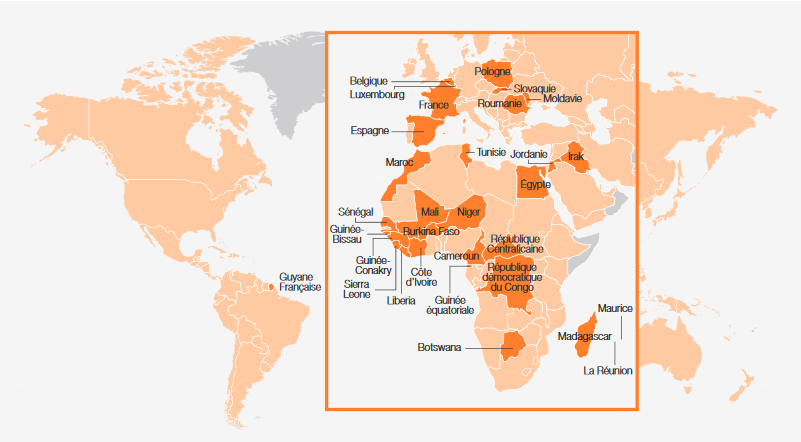
\includegraphics[scale=0.8]{./img/world_orange_2016.PNG}
    \caption{Carte des pays où est présent Orange en 2016}
\end{figure}
\paragraph*{}
Le groupe Orange est majoritairement présent en Europe et Afrique. Il est avant tout un leader de la téléphonie mobile avec un total de 202 millions de clients mobile en 2016 au niveau mondial. Orange est aussi leader dans le domaine de l’accès à Internet avec 18 millions de clients Internet haut débit fin 2016, 265 000 clients \gls{ftth} et 42 millions de clients sur la téléphonie fixe fin 2014 en France. Les pays où le groupe est le plus implanté sont la France, l’Espagne, la Pologne et la Roumanie. Depuis plusieurs années maintenant Orange essaie de se développer également en Afrique dans le domaine de la téléphonie mobile.
\paragraph*{}
Le secteur d’activité principal du groupe Orange reste les Télécommunications, en étant un opérateur téléphonique majeur en France et dans bien d’autres pays tels que la Pologne, l’Espagne, la Roumanie, Côte d’Ivoire, Égypte etc. Orange est également un fournisseur d’accès Internet et depuis quelques années élargit ses activités à la domotique, vente de contenus cinématographique et musical, médical, applications bancaires et automobiles etc.
\paragraph*{}
Les principaux concurrents d'Orange en France dans le domaine \gls{fai} sont principalement Free, Numéricâble, OVH, Nerim, Wifirst et Bouygues Télécoms. Et pour la téléphonie mobile ses principaux concurrents sont SFR, Free et Bouygues Télécom. Tandis qu'au niveau européen sur le domaine téléphonique et \gls{fai}, les principaux concurrents sont Deutsche Telekom, Vodafone et O2 en grande majorité.
\paragraph*{}
La branche où j’effectue mon alternance depuis 3 ans est \gls{ols}. Cette branche concerne tous ce qui touche à la recherche et au développement des produits Orange. Anciennement nommé France Télécom R\&D, puis \gls{olps} en 2007, et enfin rebaptisé \gls{ols} en 2017. Cette branche destinée à la recherche de l’ensemble du groupe Orange emploie 3500 personnes exclusivement en France. Fin 2012, le nombre de brevets déposés par Orange Labs s’élevaient à 7493. La R\&D est très importante pour Orange qui investit chaque année près de 900 millions d’euros dans ce secteur. \\

\subsection{Le contexte}
\subsubsection{Le Device Mangement à Orange}
\paragraph*{}
Mon alternance se déroule plus précisément au sein de l’équipe \gls{care}  qui s’occupe de la gestion des équipements client, c’est-à-dire du « Device Management ».
\paragraph*{}
Le concept de « Device Management » possède plusieurs définitions selon les objets ou équipements gérés, et les équipes qui le mettent en place. Pour nous, le Device Management s'articule autour de quatre axes:
\begin{itemize}
\subparagraph*{}
\item Provsioning: Active ou désactive un service pour le client sur l'équipement adéquate; Applique le bon \gls{firmwareg} selon le service souscrit; Paramètre de manière personnalisé la configuration d'un équipement donné en fonction des service.
\item Assistance: Permet de diagnostiquer à distance un incident sur l'équipement; Déclencher à distance l'exécution d'action permettant de corriger un incident.
\item Tracking: Collecte et stocke des informations sur l'ensemble du parc client.
\item Maintenance: Permet la mise à jour de \gls{firmwareg} à différent temps souhaité.
\end{itemize}
\paragraph*{}
L'architecture du Device Management est découpé en deux zones détaillées comme suis : 
%Import Images
\begin{figure}[!ht]
    \center
    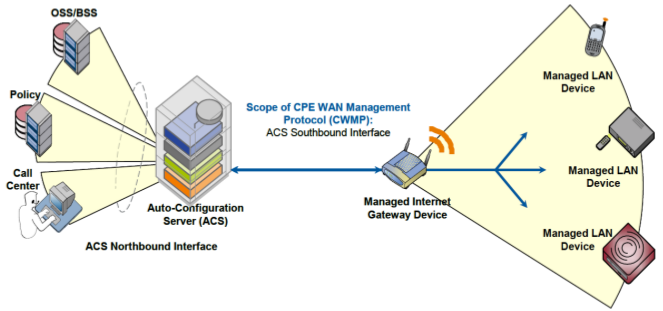
\includegraphics[scale=0.75]{./img/DM-TR-069-screen.png}
    \caption{Réseau de Device Management, côté Opérateur et côté Client}
\end{figure}
\begin{itemize}
\subparagraph*{}
\item Le coté client, où l'on retrouve le réseau privé du client, dit le \gls{lan}, avec généralement divers équipements, que l'on nomme \gls{cpe}, tels que, une passerelle Internet, un décodeur TV, un téléphone, une caméra \gls{ip}, des capteurs domotiques etc.
\item Le coté serveur, se trouvant chez Orange, où l'on va retrouver les serveurs, que l'on nomme \gls{acs}, qui vont permettre de faire ce que l'on nomme du Device Management.
\end{itemize}
\paragraph*{}
L’un des objectifs du Device Management, pour l’équipe \gls{care}, est d’apporter un service d’aide et de dépannage aux clients, tous en restant à distance. Dans le but de ne pas avoir à faire déplacer un technicien sur place, pour un problème qui peut être résolu à distance par l’exécution de scripts, lancement de test et analyse, correction de bug. Le rôle de l’équipe \gls{care}, est de concevoir l’intégration de ces outils qui pourront être utilisés à distance.
\paragraph*{}
La supervision et la maintenance du parc Orange sont d'autres activités dans le
périmètre de l'activité du Device Management. Ce parc contient les différents produits vendus par Orange et qu’Orange s'engage à maintenir. On comprend alors l'importance des activités de supervision et de maintenance. Pour gérer ce parc, Orange a besoin, entre autres, d'identifier les différents équipements présents et d'accéder à leurs  caractéristiques. Les outils de Device Management  développés au sein de l'équipe \gls{care} permettent, cette fois, de remonter aux \gls{acs} toutes les informations nécessaires pour superviser et maintenir le parc. Il permet également de mettre à jour et corriger des bugs en envoyant de nouvelles versions de \gls{firmwareg} aux équipements concernés. \\
\subsubsection{Document TR-069 et protocole normalisé CWMP}
\paragraph*{} 
Avant de continuer, il est important de préciser quelques élèments de vocabulaire propre au Device Management et décrire plus en détail comment \gls{acs} et \gls{cpe} communiquent.
\paragraph*{}Les interactions entre \gls{acs} et \gls{cpe} sont standardisées par le \gls{doctr069g}. Ce document permet, entre autre, de décrire comment implémenter la norme TR-069 sous la forme du protocole \gls{cwmp}, tant sur les \gls{acs} que sur les \gls{cpe}.
\paragraph*{}
Ce \gls{doctr069g} est le résultat d'un consortium de plusieurs industriels. Le consortium, appelé le \gls{bbf}, ce compose de plus d'une centaine de membres dont Orange, CISCO, Deutch Telecom, Huawei, Juniper, le gouvernement du Canada, Intel et bien d'autre. Le \gls{bbf} vise à décrire la gestion des équipements clients, dit \gls{cpe}, par les serveurs de gestion d'équipements, dit \gls{acs}. C'est par le \gls{doctr069g} que le \gls{bbf} décrit un standard permettant la communication entre \gls{cpe} et \gls{acs} pour une bonne gestion des équipements clients.
\paragraph*{} 
Ce standard décrit un modèle de donnée, que l'on nomme \gls{datamodelg}, comportant une partie commune pour chaque équipement implémentant le \gls{doctr069g}. Le management d'un équipement par un \gls{acs} repose en partie sur la présence de ce \gls{datamodelg}. Le standard décrit également différentes méthodes, que l'on nomme RPC Methode, obligatoire ou facultative, qui doivent être implémentées soit par l'\gls{acs} soit par le \gls{cpe}. Ces RPC Méthodes vont permettre la communication entre \gls{acs} et \gls{cpe}, et c'est de cette façon que l'\gls{acs} va pouvoir manager ses \gls{cpe}. Les RPC Methodes sont visibles en annexe.
\paragraph*{} 
Plus précisément, un \gls{cpe}, afin de pouvoir échanger avec un \gls{acs}, doit implémenter le \gls{doctr069g} sous la forme d'un client \gls{cwmp}. Les échanges \gls{cwmp} sont transportés sur du \gls{http} et encapsulés dans des messages SOAP. La création d'une session \gls{cwmp} ce fait toujours par le \gls{cpe}. L'\gls{acs} ne peut pas créer de session, en revanche il possède différentes techniques lui permettant de demander au \gls{cpe} de venir initialiser une session \gls{cwmp}. \\

\subsection{Objectifs}
\paragraph*{}
Au cours des trois années passées dans l'équipe \gls{care}, il m'a été confié différents objectifs d'importance et de responsabilité croissante. Ces objectifs m'ont permis de monté en compétences tant sur l'aspect technique que l'aspect transversal du métier d'ingénieur informatique.\\
\subsubsection{Première année}
\paragraph*{}
blabla
\\
\subsubsection{Deuxième année}
\paragraph*{}
blabla
\\
\subsubsection{Troisième année}
\paragraph*{}



\newpage
\section{Monté en compétence sur le protocole CWMP}
\subsection{Études d'équipements}
\subsubsection{Présentation du réseau isolé}
\subsubsection{Test DNS}
\subsubsection{Test de comportement TR-069 d'équipement}
\subsection{Étude de client CWMP}
\subsubsection{Client EasyCWMP}
\subsubsection{Client tr69agent d'Orange}
\subsubsection{Résultats} %conséquence : création du toolkit !
\subsection{Création d'un ACS Servlet}
\subsection{Impact sur mon parcours}


\newpage
\section{Conception et développement de TINK}
\subsection{Contexte}
\subsection{Présentation}
\subsection{Méthode de projet}
\subsection{Travail de préparation}
\subsubsection{Recherche de solution technique}
\subsubsection{Analyse de faisabilité}
\subsection{Conception}
\subsection{Réalisation}
\subsubsection{Travail en équipe}
\subsubsection{Développement}
\subsection{Déploiement}
\subsubsection{Environement}
\subsection{Communication et utilisateur}
\subsection{Livrable du projet}
\subsection{Difficultés, solutions et compétences acquises}
\subsection{Bilan et apport personnel du projet}

\newpage
\section{Transfert de compétences}

\newpage
\section{Bilan de compétences} 
\subsection{Environnement professionnel}
\subsubsection{Connaissance de l'entreprise}
\paragraph*{}Lors de mon arrivée au sein de l'entreprise, une présentation des différents services avec lesquels j'étais susceptible de travailler m'a été faite. Cela m'a permis dans un premier temps d'avoir une connaissance partielle des ressources humaines avec lesquelles je serais amené à travailler tout au long de mes trois années de formation. Grâce à cette connaissance de l'environnement de travail, j'ai pu savoir qui contacter directement en cas de besoins dans de nombreuses situations. Notamment, lorsque j'ai débuté certains projets, comme je savais que certaines personnes avaient au par-avant abordées des sujets similaires ou dans des domaines équivalents, cela m'a permis d'obtenir davantage de connaissances pour les sujets sur lesquels j'allais être amené à composer. De la même façon, lorsque j'ai rencontré des points bloquant sur la partie technique, j'ai su quelles personnes contacter afin de pouvoir monter en compétences plus rapidement dessus afin de résoudre la difficulté. \\
Enfin, si au cours de ma première année j'ai souvent eu à contacter différentes personnes pour leur demander des informations ou de l'aide, j'ai vu durant la deuxième année l'inversion progressive des rôles. En effet, des personnes sont venues me demander des renseignements ou une seconde analyse sur leurs résultats. \\
\subsubsection{Anglais et contexte international}
\paragraph*{}Mes activités et projets de première année ne pas permis d’interagir avec des équipes internationales. Cependant, lors de ma deuxième année j'ai été amené à travailler avec un membre d'une équipe de conception et développement roumaine. Ce travail en collaboration a eu pour conséquence de me faire monter en compétence non pas uniquement sur l'aspect technique, mais aussi sur mon anglais écrit, puisque nous échangions en anglais par écrit le plus souvent. \\
De plus, durant ces deux premières années j'ai pu traiter et rédiger de nombreux documents en anglais. Lors de mon arrivée au sein de l'équipe, il m'a été aussi demandé de lire plusieurs documents techniques concernant le domaine dans lequel j'allais évoluer et travailler. L'ensemble de ces documents était rédigé pour la majorité en anglais, ce qui fut pour moi l'occasion d'acquérir des notions en anglais technique. Dans un second temps, j'ai eu à rédiger des documentations et participer à la rédaction de wiki de mon projet de deuxième année. Ces rédactions ont été un moyen de mettre en pratique les notions d’anglais précédemment acquises. Depuis la deuxième année il m'a été en plus demandé de rédiger un cahier des charges ainsi qu'un dossier de spécification intégralement en anglais. Cela m'a ainsi permis de monter en compétence en anglais technique tout au long de ces deux ans. \\

\subsection{Management}
\subsubsection{Travail en équipe et communication}
\paragraph*{}Les premières missions qui m'ont été confiées n'impliquaient pas de travail collaboratif. Je devais faire des rapports à mon tuteur, selon l'avancée du projet. Ce dernier supervisait alors mes missions, en me laissant toutefois déjà une importante autonomie. Lors de réunion ayant lieu toutes les deux semaines, je présentais mon avancée de manière plus synthétique au reste de l'équipe. J'ai ainsi pu acquérir des notions en communication, ainsi que dans les compétences de restitution et présentation orale. \\
C'est dans la seconde moitié de ma première année que j'ai pu travailler sur des missions impliquant d'autres collaborateurs. Ce fut pour moi l'opportunité d'apprendre à organiser mon travail en prenant en compte également celui de mes collègues. Pour ce qui est de l'aspect communication, cela m'a permis de renforcer mes compétences en relatant mon travail lors des points d'avancés, mais aussi en étant force de proposition lors des réunions de travail où j'exprimais mon opinion sur les solutions envisagées et proposais d'autres possibilités. \\
Mon attitude professionnelle et l'évolution de mes compétences en travail d'équipe et en  management ont conduit mon tuteur à me confier l'encadrement partiel d'un stagiaire de Master 2 sur la seconde moitié de ma deuxième année. Il m'a été demandé de l'encadrer durant mes périodes en entreprise en répartissant entre nous les tâches composant le projet sur lequel nous travaillons. Cet exercice m'a permis de renforcer davantage ma communication et ma gestion du travail en équipe, en planifiant des réunions et des points d'avancement, ainsi qu'en assignant des activités au stagiaire. Cet exercice s'étant bien déroulé, mon tuteur a décidé de me confier l'encadrement intégral d'un stagiaire de dernière année de cycle d'ingénieur lors de ma dernière période de troisième année. \\
\subsubsection{Gestion du temps et du stress}
\paragraph*{}Les missions qui m'ont été confiées tout au long des six premiers mois de ma formation n'impliquaient pas de date limite de rendu de projet. J'ai cependant eu besoin d'organiser mon travail et gérer le temps que je passais sur chacune de mes activités. Tout au long de la première année mon travail fut partagé entre deux activités principalement. Même si ces activités n'incluaient pas toujours un travail en collaboration, cela a tout de même nécessité l'organisation et la planification de mes temps de travail et actions sur chacune de ces deux activités. Cela m'a permis d'acquérir des notions dans ma gestion du temps. \\
Ce n'est qu'à partir de la seconde moitié de ma deuxième année que des contraintes de date limite m'ont été imposées. Cela fut notamment dans le cas dans le projet qui a occupé l'intégralité de cette année, où différents jalons avaient été définis soit initialement, soit au cours du projet. J'ai alors mis en place des outils d’organisation afin de gérer mon temps de manière plus efficace et renforcer encore mes compétences dans ce domaine. J'ai appris à estimer la priorité, la complexité et le temps de réalisation de différentes actions, dans le but d’estimer de la façon la plus efficace possible le temps de travail nécessaire à la réalisation de ces actions. \\
L'apparition des dates limites et des enjeux à finir une activité dans le temps imparti m'a permis d'apprendre à gérer également mon stress. \\

\subsection{Conduite de projet}
\subsubsection{Analyse des besoins}
\paragraph*{}Les premières missions qui m'ont été confiées à mon arrivée au sein de l'équipe n'impliquaient pas de réelle analyse des besoins. En revanche, à partir de la seconde partie de la première année, j'ai eu progressivement des projets nécessitant que je recueille des besoins, fonctionnalités et critères essentiels pour mener à bien mes projets. Dans un premier temps cela consistait essentiellement à poser les bonnes questions à mon tuteur, qui m'avait attribué le projet. Progressivement j'ai eu à réaliser des études de faisabilités afin de démontrer que mes solutions étaient viables, ou tout simplement pour sélectionner la solution la plus adéquate au problème posé. \\
Mon tuteur m'a confié progressivement des missions qui nécessitaient une réflexion plus approfondie sur la recherche de solutions techniques et sur l'analyse de besoins, à partir de la seconde partie de ma première année. Afin que je puisse réaliser ce travail correctement lors de ma deuxième année. L'une des phases de mon projet de deuxième année consistait justement à définir et décrire les besoins, puis réaliser une étude de faisabilité de manière la plus autonome possible puisque mon tuteur souhaitait que je réalise ces étapes moi-même tout en étant capable d'argumenter mes choix. Le fait d'avoir eu à examiner et à décomposer le projet en intégrant différents paramètres m'a permis d'avoir une certaine prise de recul sur ce que l'on me demandait de réaliser. \\
\subsubsection{Planification et méthode de gestion de projet}
\paragraph*{}Dès ma première année j'ai eu à planifier mes activités. Mais c'est à partir de ma deuxième année que j'ai vraiment pu utiliser des méthodes de projet, notamment l'agilité avec les méthodes Scrum et Kanban. Ces dernières m'ont permis d'organiser et préparer au mieux mon projet et mon travail collaboratif, puisque de cette façon je savais où en étaient mes collaborateurs dans leurs tâches sur le projet. Le fait de mettre en place une méthode de projet m'a permis d'apprendre à décomposer le travail et à pouvoir le répartir entre les différents membres de manière égale et la plus adéquate possible en fonction des compétences de chacun.\\
Monter en compétence sur la gestion de projet et sur la décomposition des tâches m'aide à préparer au mieux mon travail et avoir une meilleure visibilité sur celui-ci. \\
J'ai de plus été amené à rédiger un dossier de spécification pour mon projet de seconde année, constitué d'un cahier des charges ainsi que de plusieurs diagrammes UML. Cet exercice de rédaction permet d'avoir encore une fois une meilleure vue sur ce qui est attendu, de son contexte et des différentes étapes. \\

\subsection{Systèmes d'Information}
\subsubsection{Architecture logicielle}
\paragraph*{}Durant ma première année j’ai pu, dans le cadre du projet de première année, concevoir une application utilisant l’architecture logicielle MVC (Model View Controller). Cela m’a permis d’acquérir des notions dans le domaine de patron de conception. Mon tuteur m’a également encouragé à utiliser d’autre patron de conception lors de l’un de mes projets qui nécessitait que je conçoive une application et donc son architecture. \\
Lors de ma deuxième année, mon tuteur m'a confié la conception, puis le développement, d'un outil plus complexe que ce que j'avais pu réaliser jusqu’à présent. Cela a nécessité de ma part de prendre connaissance de plusieurs types d'architectures logicielles existantes. À savoir l'architecture n-tiers; comprendre chacune de ces couches qui composent cette architecture; leurs rôles et leurs fonctionnements. De plus, j'ai eu besoin de comprendre comment faire communiquer les différents modules de cette architecture, tout en prenant en compte les contraintes et les besoins impliqués dans le projet. Cela a nécessité de ma part de questionner à la fois des collaborateurs, développeurs seniors, ayant un niveau de compétences avancé dans l'architecture de logiciels. Le fait d'avoir pu contacter des développeurs seniors m'a permis de monter en compétence et d'avoir une importante source de connaissances à disposition. J'ai également récupéré les cours donnés aux étudiants INFRES ED de deuxième année qui abordent ce sujet, ce qui m'a permis d'acquérir d'autres notions. \\
J'ai ainsi pu concevoir l'architecture logicielle d'une application, basée sur une architecture n-tiers, tout en prenant en compte les évolutions futures et la maintenabilité de celle-ci. Cela m’a permis de monter en compétence dans les architectures logicielles.\\

\subsection{Logiciels}
\subsubsection{Conception et développement d'applications}
\paragraph*{}Lors de mon arrivée dans l’entreprise, mon tuteur m’a fait travailler sur l’étude d’un client embarqué développé en C. Cela dans le but de me faire monter en compétence en développement C, puisqu’il m’a fallu comprendre le fonctionnement de ce client  à l’aide de reverse-engineering. Cela avait aussi pour but de me donner des notions en conception d’applications, en devant essayer de comprendre comment ce client avait était conçu. Puis dans un second temps, le modifier afin d'étudier la complexité à rajouter des fonctionnalités. Cette seconde phase m'a permis de mettre en application mes compétences en développement C mais aussi en conception. \\ 
Dans la seconde partie de ma première année, afin d’acquérir des notions supplémentaires dans la conception d’application, mon tuteur m’a fait travailler sur la conception d’un outil doté de fonctionnalités simples. La conception de cette application avait pour second objectif de me faire rentrer davantage dans le domaine d’activité sur lequel j’allais travailler durant mes trois ans de formation, en utilisant des concepts de cet outil. Cela m’a permis de monter à la fois en compétence sur les aspects de bases de conceptions d’applications, mais également de renforcer mes compétences en développement, particulièrement sur le langage orienté objet Java. \\
Lors de ma deuxième année, il a été décidé de me faire concevoir et développer un outil plus complexe que l’application implémentée en première année. Ce projet devait occuper l’ensemble de la deuxième année, et une partie de la troisième. De plus, le travail de conception a été réalisé en travail collaboratif avec un second collègue. J’ai également pu demander des conseils, des explications et des aides à différents développeurs seniors pour la conception de cet outil. De plus le développement de celui-ci s’est effectué en Java et m’a permis de travailler avec de nombreux frameworks fréquemment utilisés et relativement complexes à prendre en main. Le fait d’avoir pu apprendre à utiliser ces frameworks m’a permis d’acquérir de solides bases et compétences en développement Java. \\
De part la conception, l’étude et le développement de ces différentes applications, dans les langages C et java, j’ai pu monter en compétence dans la conception logicielle et le développement d’applications.\\

\subsection{Systèmes et Réseaux}
\subsubsection{Administration et maintenance d'OS}
\paragraph*{}Depuis le début de ma formation je travaille la majorité de mon temps sur des machines Linux, ce qui favorise le développement de mes compétences d'administration OS Linux et le langage orienté OS associé. De plus, lors de ma première année j'ai eu à recréer un réseau opérateur dans le cadre de tests d’équipements. Pour cela il m'a fallu configurer différents services et serveurs, me permettant de renforcer mes compétences en administration de système. J'ai par ailleurs eu à configurer et déployer des serveurs d'applications dans le cadre de ma deuxième année, ce qui a là encore pu renforcer mes compétences dans ce domaine acquis une première fois lors de mon DUT, mais aussi lors des cours de deuxième année que nous avons pu avoir. \\
Mon tuteur souhaite désormais que pour ma troisième année je participe à la sécurisation d'un serveur de production afin de monter en compétence dans la sécurité d'un point de vue administrateur système. Durant les périodes d'école de ma deuxième année j'ai également pu monter en compétence en administration d'OS, tant Linux et Microsoft, grâce aux différents cours qui m'ont été donnés. \\  
\subsubsection{Protocole de Communication}
\paragraph*{}Tout au long de ma formation, mon domaine d'activité en entreprise implique que j'ai une forte connaissance d'un protocole de communication client/serveur, nommé CWMP. Ce protocole est une importante brique de l'ensemble de mes projets. Il m'a donc été nécessaire de monter rapidement en compétence sur ce protocole dès mon arrivée dans l'entreprise. L’apprentissage de ce protocole m'a permis de monter en compétence dans mes connaissances des protocoles de communication. \\

\subsection{Axe d'amélioration}
\paragraph*{} Ainsi que l'on peut le voir ci-dessous avec le \textit{Tableau d'auto-évaluation de compétences}, il y a de nombreuses compétences qui n'ont pas pu être encore développées. Cela s'explique par les sujets couverts jusqu'à présent lors des cours proposés à l'école, ainsi qu'aux missions effectuées en entreprise, qui ne peuvent bien évidemment pas couvrir l'ensemble des domaines du référentiel de compétence. Il est donc normal de voir des compétences plus avancées que d'autres, puisque l'on ne peut pas travailler sur toutes. Toutefois, il me semble intéressant pour mon futur professionnel de renforcer davantage mes compétences dans les domaines de \textit{Systèmes et Réseaux}, \textit{Conduite de projet} et \textit{Systèmes d'Information}. Ces différents domaines feront l'objet, en partis de ma troisième année ce qui me permettra de renforcer mes compétences dans ces domaines. \\

\subsection{Conclusion}
Comme nous avons pu le voir tout au long de ce document, ma première année fut pour moi riche en matière d'acquisitions de bases et notions dans de nombreux domaines de compétences. La seconde année m'a permis de renforcer ces compétences en améliorant ma manière de travailler, d'appréhender un problème, ou encore de faire face à un problème. Durant cette deuxième année, j'ai pu acquérir de nouvelles compétences, qui seront elles aussi renforcées durant ma dernière année. Ces différentes phases d'acquisitions des compétences de l'ingénieur tendent ainsi à me rapprocher davantage du statut d'ingénieur souhaité par l'école. 

\newpage
\section{Conclusion}
\subsection{Atteintes des objectifs}
\subsection{Progression}
\subsection{Synthèse de parcours}


\newpage
%ANNEXE
\begin{appendix}
\chapter{RPC Method CWMP}
\begin{table}
	\begin{tabularx}{17cm}{|l|X|}
		\hline
		RPC Method & Description\tabularnewline
		\hline
		InformResponse & Permet à l'ACS de répondre à un Inform.\tabularnewline
		\hline
		GetParameterValues & Permet de récupèrer la valeur d'un ou plusieurs 				paramètre du datamodel passé en paramètre.\tabularnewline
		\hline
		SetParameterValues & Permet de modifier la valeur d'un ou plusieurs 				paramètre du datamodèle passé en paramètre.\tabularnewline
		\hline
		Reboot & Permet à l'ACS de demander au CPE de redémarrer.\tabularnewline
		\hline
		FactoryReset & Permet à l'ACS de demander au CPE de se réinitilisaer à l'état d'usine.\tabularnewline
		\hline
		ScheduleInform & Permet à l'ACS de demander au CPE de revenir initilisaer une session TR-069 dans t seconds.\tabularnewline
		\hline
		Download & Permet à l'ACS de demander au CPE de télécharger un fichier, souvent un nouveau firmware.\tabularnewline
		\hline
	\end{tabularx}
	\centering
	\caption{Liste des RPC méthodes devant être implémentées par l'ACS.}
\end{table}
\begin{table}
	\begin{tabularx}{17cm}{|l|X|}
		\hline
		RPC Method & Description\tabularnewline
		\hline
		Inform & Permet au CPE d'initier une session TR-069.\tabularnewline
		\hline
		GetParameterValuesResponse & Permet au CPE de répondre à un 						GetParameterValues en indiquant la/les valeur(s) du/des paramètre(s) 				demandé(s) par l'ACS.\tabularnewline
		\hline
		SetParameterValuesResponse & Permet au CPE de répondre à un 						SetParameterValues en indiquant si la demande a pu être réaliser.\tabularnewline
		\hline
		RebootResponse & Permet au CPE d'acquitter l'ordre de redémarrage.\tabularnewline
		\hline
		FactoryResetResponse & Permet au CPE d'acquitter l'ordre de réinitilisation à l'état d'usine.\tabularnewline
		\hline
		ScheduleInformResponse & Permet au CPE d'acquitter l'ordre de ScheduleInform.\tabularnewline
		\hline
		DownloadResponse & Permet au CPE d'acquitter l'ordre de Download.\tabularnewline
		\hline
	\end{tabularx}
	\centering
	\caption{Liste des RPC méthodes devant être implémentées par le CPE.}
\end{table}

\chapter{Tableau d'auto-évaluation de compétences}
%Import Images
\begin{figure}[!ht]
    \center
    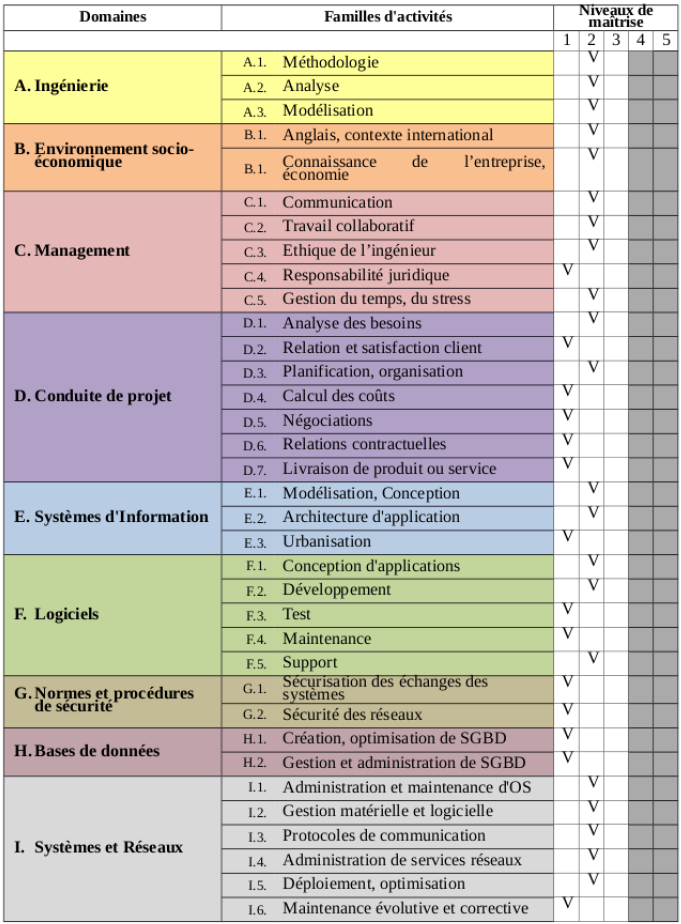
\includegraphics[scale=0.9]{./img/tableaux_cpt.PNG}
    \caption{Tableau d'auto-évaluation des compétences}
\end{figure}

\end{appendix}
\end{document}
